\section{Native Token: \$ZOO}
\label{sec:native-token}

\textit{An exceptional digital asset backed by gold and silver, \$ZOO is the native token for the Zoo Game.}

\subsection{Gold- and Silver-Backed Token}

The Zoo Token forms the core of the Zoo ecosystem, distinctively characterized by its unique backing of gold and silver. It is not merely a digital asset but a gateway to the physical commodities realm, creating an innovative fusion of traditional and crypto assets.

The Zoo Token's distinctiveness starts with its multiplicity of liquidity pools. Unlike traditional tokens that are often confined to specific pools, Zoo Token's liquidity transcends typical boundaries, promoting accessibility and versatility for token holders. The founding members of Zoo Game will launch the largest liquidity pools, which will contain Lux Tokens exclusively. These Lux Tokens, representing real-world commodities, are backed by silver and gold, infusing tangible value and stability into the digital Zoo ecosystem.

The flexibility of transactions with these Lux Tokens is key to understanding their value. Token holders have the liberty to transfer, sell, or even redeem these tokens for their physical counterparts. The Zoo Token unlocks a pathway to an assortment of natural assets and commodities. The initial phase focuses on precious metals; future phases broaden the scope to a wider array of valuable resources, further diversifying and enriching the commodities within the ecosystem.

The Zoo Token is more than a game token. It embodies a bridging function between virtual and real-world assets. This pioneering step blurs the lines between the digital and physical worlds, bringing a unique dimension of trading precious metals within the virtual Zoo ecosystem.

\subsection{Ease of Acquisition}

Through an inventive bridge feature, the Zoo Token can be purchased with almost any asset, allowing users to effortlessly transform their existing holdings into Zoo Tokens. This level of convenience encourages a wider demographic of participants to engage within the Zoo ecosystem, fostering inclusivity. Zoo Labs capitalizes on its gold-backed token expertise to design a solid framework for the implementation of commodity-backed tokens, catering to a spectrum of participants --- crypto enthusiasts seeking innovation and traditional investors seeking tangible assets with a secure store-of-value function.

\section{Collateral-Backed NFTs}
\label{sec:collateral}

\begin{figure}[h]
  \centering
  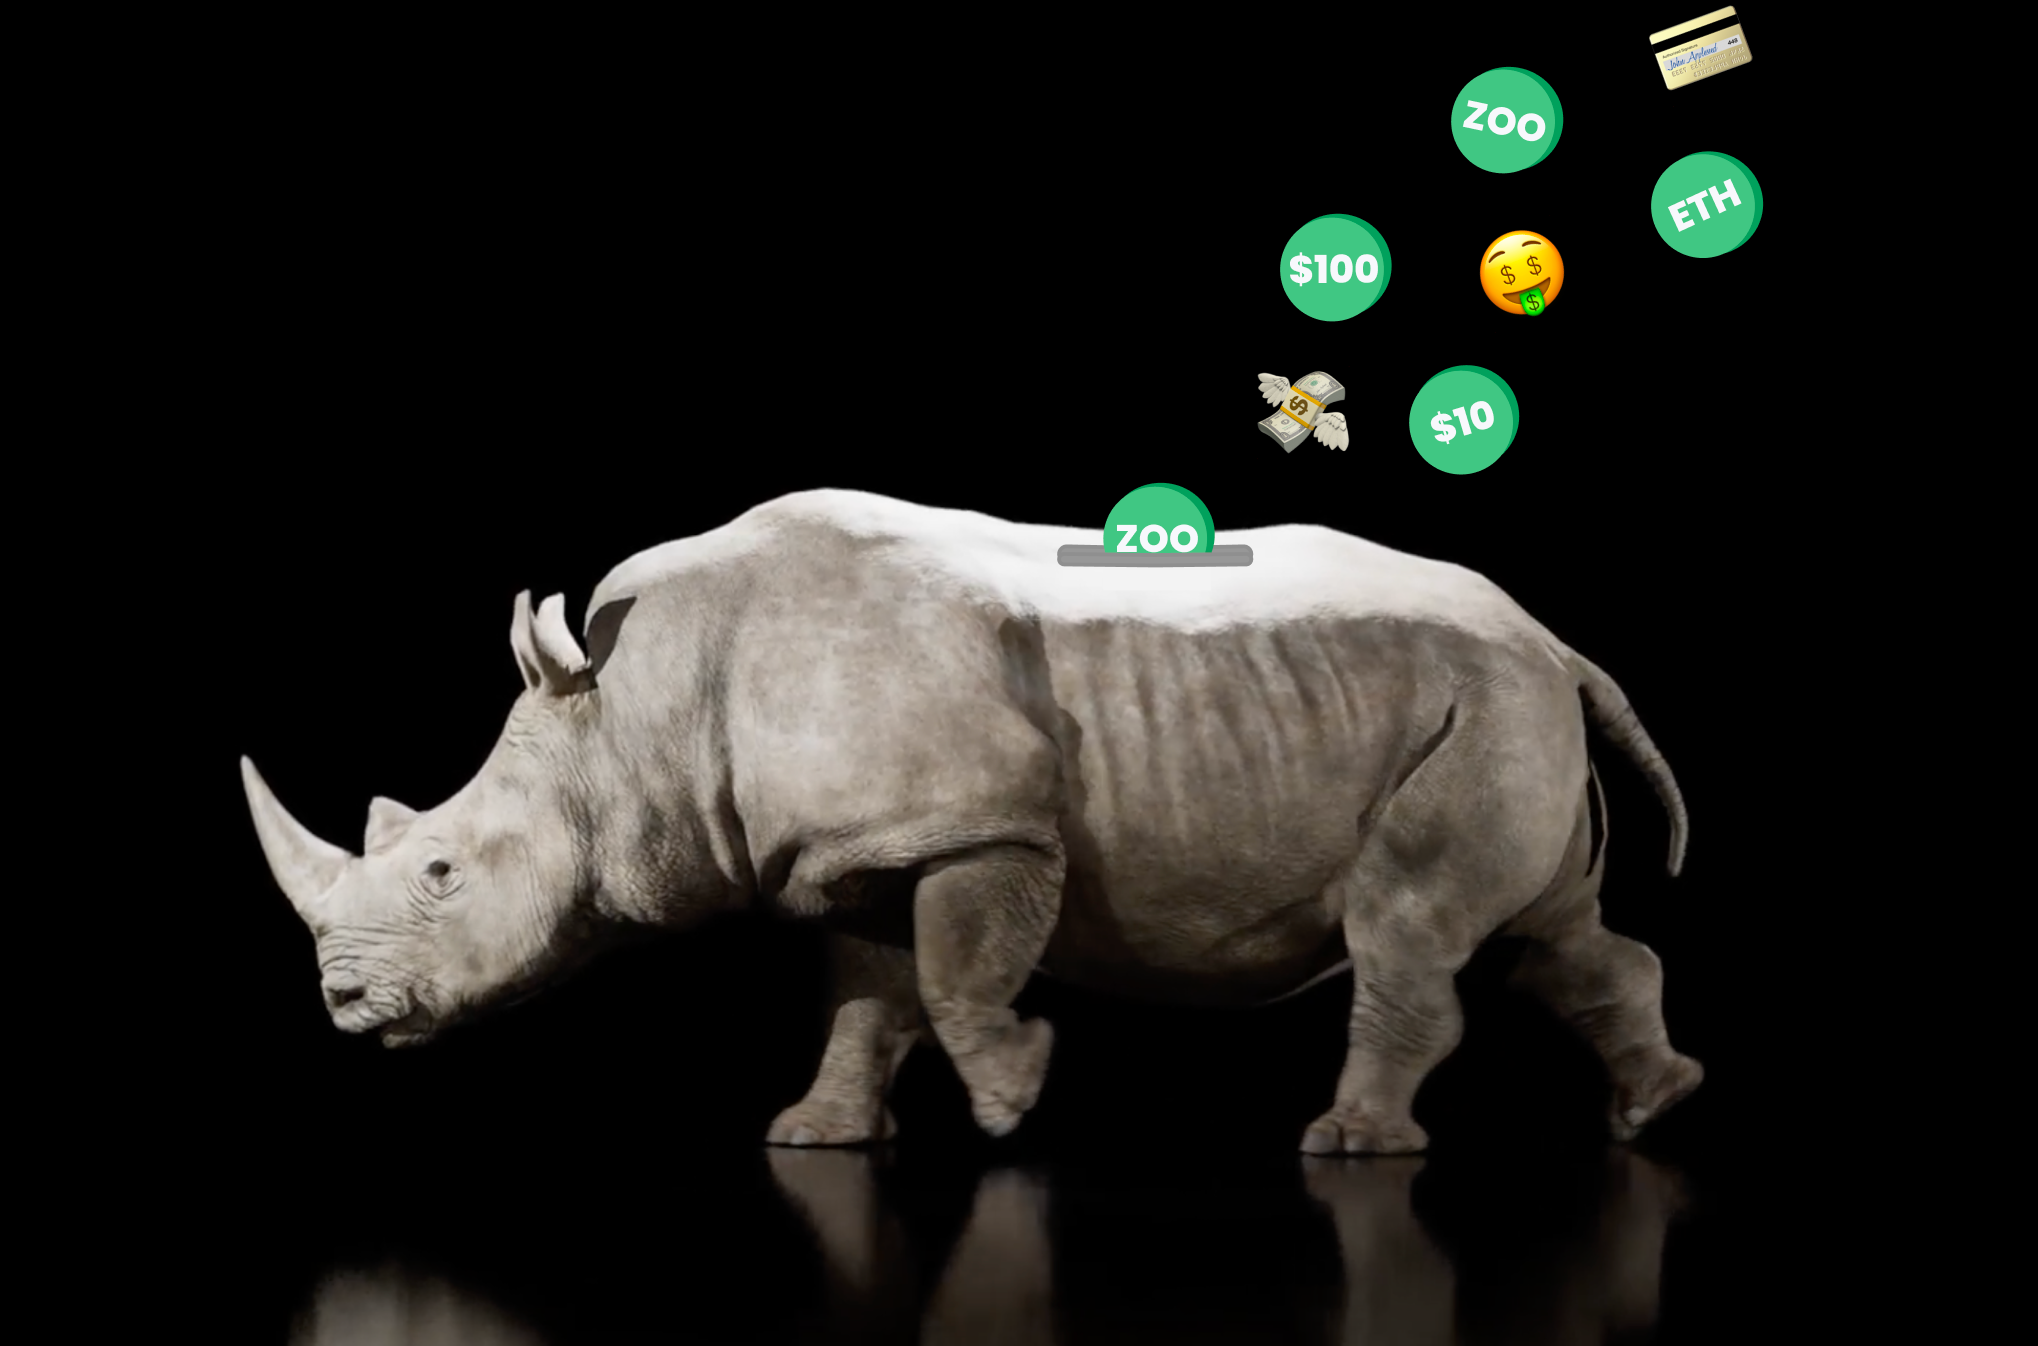
\includegraphics[width=0.85\linewidth]{figures/collateral.png}
  \caption{The collateral mechanic: NFTs serve as ``piggy banks'' that lock in staked value, earning APY based on rarity. Releasing collateral requires either selling on the marketplace or burning the NFT.}
  \label{fig:collateral}
\end{figure}

\subsection{Staked Collateral}

As you collateralize your animal NFT or egg, you are locking value into your NFT. The NFT's intrinsic value is based on its scarcity, and your collateral is multiplied by the APY of your animal for additional rewards. You can typically resell the NFT for a higher value than the price purchased plus your collateral plus your rewards earned. Or you can simply burn the NFT and get back the collateral value plus the rewards. The only ways to retrieve staked collateral and rewards earned are to burn the NFT or sell it on the Zoo Marketplace.

Zoo is designed to easily add collateral or stake any currency on any of the Zoo Labs NFTs by feeding, breeding, or by minting an older NFT version of the animal.

\subsubsection{Releasing Collateral}

Once a user stakes collateral into their NFT, that value is locked in --- deposited into our cute NFT animal piggy banks. The collateral earns APY based on the NFT's rarity, which determines the reward yield rate. As rewards accrue, they become part of the collateral, increasing the NFT's reward base. To liquidate collateral and rewards, the user has two options:
\begin{enumerate}[label=(\alph*)]
  \item Sell and transfer the NFT animal for the value of the NFT plus its intrinsic value. Selling on the marketplace returns the staked value and provides the opportunity to make more based on intrinsic value (rarity-driven).
  \item Burn the NFT, returning staked value plus rewards earned to date. When burned, the allotment to mint older animals (if possible) is gone forever, removing one of its species from the deflationary ecosystem. A 20\% sustainability tax applies on burn: 10\% to the DAO and 10\% back to the liquidity pool.
\end{enumerate}

\subsubsection{Rewards}

Every NFT is a representation of an endangered species. The ecosystem represents the animal kingdom of endangered species --- over 18{,}000 of them. The number of NFTs we release into circulation is dependent on how rare and endangered these animals are in the real world. Our first drop consists of 1{,}800 hatchable eggs across three rarity tiers. These NFTs earn rewards and extra boosts on collateral staked. When hatched, each egg reveals an animal which earns rewards for a year.

\subsection{Feeding (a.k.a.\ adding Collateral)}

First you incubate an egg, which hatches into an Origin Baby Animal. Similar to Tamagotchi, users can ``care'' for their pets by feeding them and watching them age up. Feeding is defined as adding any currency to the NFT, locking it in until the user decides to burn or sell. Continued feeding eventually mints the older versions; the user just has to feed it the same value as its base cost.

There are seven generations of NFTs in the Zoo ecosystem. It starts with an egg, then a baby, a teen, and finally an adult. If a user collects two adults of the same species, they can breed them to mint a new baby animal. Each Origin Egg can mint 1{,}500+ animals. Origin animals can breed seven times; each subsequent generation has one less breed available. The ultimate objective of the game is to collect the highest yielding and most rare NFT within the Zoo ecosystem.

\subsection{Boosts}

Boosts amplify the daily reward according to collateral staked.
\begin{itemize}
  \item \$10--\$99: \textbf{1.1$\times$}
  \item \$100--\$999: \textbf{1.2$\times$}
  \item \$1{,}000--\$9{,}999: \textbf{1.3$\times$}
  \item \$10{,}000+: \textbf{1.4$\times$}
\end{itemize}

\subsection{Breeding}

NFT animals can be bred with other NFT animals once they reach their adult form, achieved by feeding the NFT animal a specified amount of crypto. Each NFT animal can be bred up to seven times; you may breed any two adult animals of the same species to produce an NFT egg. The result is a totally random NFT egg from that drop, including potentially the rarest. To breed two adult NFT animals, the user selects each animal in the d'App UI, then initiates the process by feeding the designated amount of \$ZOO tokens. This mints a random NFT egg, which can be sold, transferred, or incubated and hatched.
